\chapter{Vehicle Detection Module}  \label{kap:vehicle-detection}

\section{Classification refinement} % (fold)
\label{sec:Classification-refinement}

Due to the great spectrum of different textures appearing in an image, false
classification may occur. This is essentially an inherent problem of the
effort the classifier does to predict unknown data. These mistakes from the
classifier are divided into two types, false positives and false negatives. A
false positives occur when the classifier wrongly label negative examples as 
positive and false negatives is the other way around.

Sometimes it is possible to use some strategies to improve a classification by
removing some of this false classifications. In this particular project, we have
the advantage to work with a continuous flow of images coming from a camera.
This fact offers an extra dimension which allow us to make assumptions in
order to filter some of the false classifications.

Basically we assume the camera is fixed inside the vehicle, meaning that the images
coming from it should show always the frontal view. This summed to the stream of
images allow us to suppose that a vehicle appearing in one image is going to also 
appear in the next one, in almost the same region inside the image.

With this in mind, it is easy to design a simple strategy to eliminate some
false positives. Supposing a vehicle can not simply disappear from one
frame to the other, we can construct a classification window over time, where we
keep track of the position of all the previous classified vehicles. If a new
classification is not consistent with the previous ones in the window, then it
is simply dropped. 

The final size of the region containing the vehicle is averaged with the
information inside the classification window. This smooths jumps of the region
size returned by the classifier due to the search in different scales.

% section Classification refinement (end)


\section{Distance estimation} % (fold)
\label{sec:Distance-estimation}

When projecting the real 3D world through the lenses of a camera into a 2D
image, some information is lost. In particular, the scale and the notion of
distances is lost. It is not possible give any real
measurement of distances in the real world just looking at one image. 
Of course, as humans we can find references in an image of something we already
know and stablish some scale to compare the rest of the image. Think for
example of a picture of a small toy car. If the model of this toy car is good 
enough, a human can not differentiate it from a real one, then having an
incorrect estimate of its size.

This is the problem faced in this section and of course, it is required to do some
assumptions to be able to approximate a solution. First it is assumed, that the
pictures obtained from the camera are from real vehicles, this is really
important to build references with of real world distances. Now, this brings a
second problem, that not all the vehicles have the same size. 
The easy solution is to make a second assumption and consider an average width
of all the vehicles appearing in the images.

The third problem is that the width in meters of the vehicles is not obtained 
directly from the picture, but a group of pixels containing the image of
the car. To solve this, is necessary to find the relation between the number of
pixels containing the car, and the distance to it. For this reason, as a first
approach, a number of pictures at different distances of a car where taken. This
pictures appear in the figure [inser figure here].

In the figure~\ref{fig:distance-curve-fitting} are displayed as red points, the
measurements obtained from each image. As you can see, this points follows an
exponential function. In order to be able to make a prediction of the distance,
it was decided to fit a exponential model to this data points. The exponential
model selected for this task is given by the next formula

\begin{equation}
    \mathcal{M}(x) = a \cdot \exp(b \cdot x) + c \cdot \exp(d \cdot x)
    \label{eq:distance-curve-model}
\end{equation}

\begin{figure}[h]
\centering
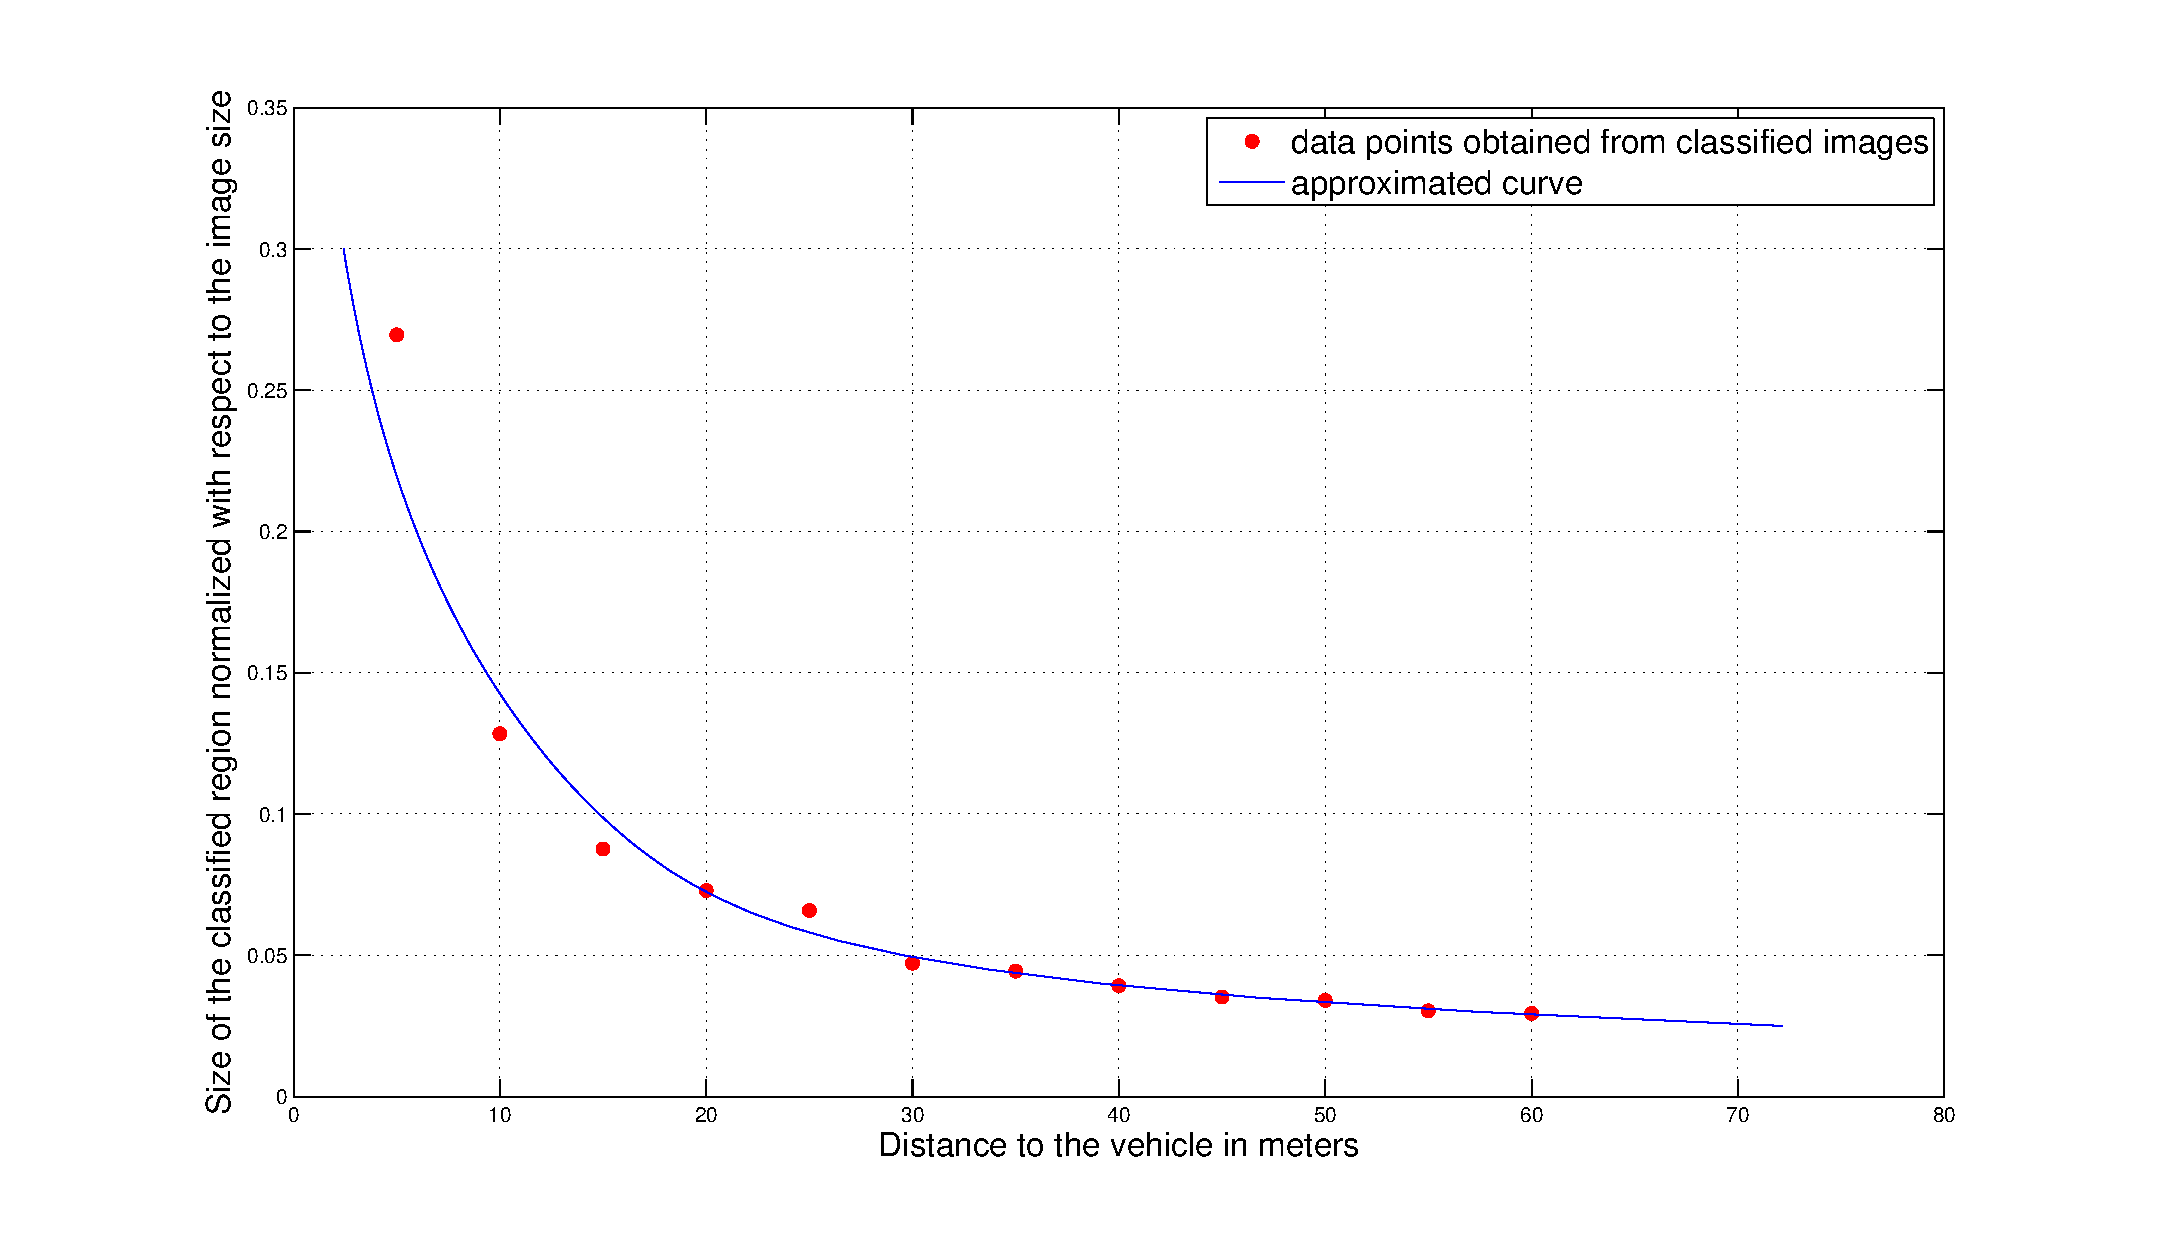
\includegraphics[width=\linewidth]{img/fitted_curve.eps}
\caption{This image shows the curve approximated to the measurements obtained
from the pictures. In the horizontal axis is the width in pixels of
the classification bounding box around the vehicle. In the vertical axis is the
distance in meters to the vehicle. The red points represent the measure obtained
from each image. The blue curve is the predicting model fitted to the data points.}
\label{fig:distance-curve-fitting}
\end{figure} 

It is important to point out that this approximated model is directly related to
the classifier itself. This is because the measurements from the pictures are
obtained through it. This implies that whenever the classifier is changed, a new
coefficients are need to be found.

These coefficients creates a relationship between the width in pixels
of the classified image of the vehicle with the distance in meters to the
vehicle in the real world. Therefore they offer an approximated distance to the
vehicle, giving an initial solution to the problem of distance estimation.

% section Distance estimation (end)
